\documentclass[tikz,border=4mm]{standalone}
      \usepackage{tikz}
      \usetikzlibrary{arrows.meta,positioning,calc,shapes.geometric}
      \begin{document}
      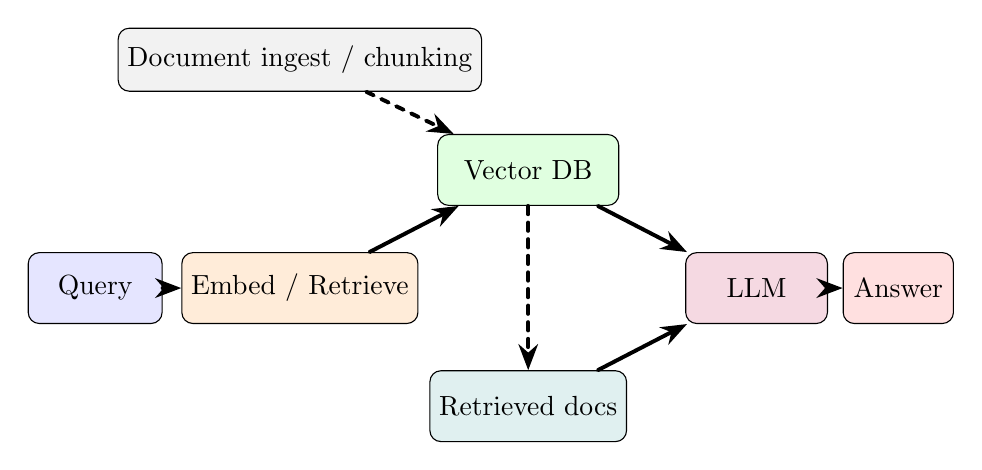
\begin{tikzpicture}[>=Stealth, line cap=round, line join=round]

\node[draw, rounded corners, fill=blue!10, minimum width=1.7cm, minimum height=0.9cm] (q) at (1.4,4.5) {Query};
\node[draw, rounded corners, fill=orange!15, minimum width=2.4cm, minimum height=0.9cm] (ret) at (4.0,4.5) {Embed / Retrieve};
\node[draw, rounded corners, fill=green!12, minimum width=2.3cm, minimum height=0.9cm] (vdb) at (6.9,6.0) {Vector DB};
\node[draw, rounded corners, fill=teal!12, minimum width=2.3cm, minimum height=0.9cm] (ctx) at (6.9,3.0) {Retrieved docs};
\node[draw, rounded corners, fill=purple!15, minimum width=1.8cm, minimum height=0.9cm] (llm) at (9.8,4.5) {LLM};
\node[draw, rounded corners, fill=red!12, minimum width=1.4cm, minimum height=0.9cm] (ans) at (11.6,4.5) {Answer};
\node[draw, rounded corners, fill=gray!10, minimum width=3.0cm, minimum height=0.8cm] (ing) at (4.0,7.4) {Document ingest / chunking};
\draw[->, line width=0.05cm] (q) -- (ret);
\draw[->, line width=0.05cm] (ret) -- (vdb);
\draw[->, line width=0.05cm] (vdb) -- (llm);
\draw[->, line width=0.05cm] (llm) -- (ans);
\draw[->, line width=0.05cm, dashed] (ing) -- (vdb);
\draw[->, line width=0.05cm, dashed] (vdb) -- (ctx);
\draw[->, line width=0.05cm] (ctx) -- (llm);

      \end{tikzpicture}
      \end{document}
